\begin{frame}
 \frametitle{Erstellen von Prädiktoren}
 \framesubtitle{PCA - Principal Component Analysis}
 Ziel: Dimensionsreduktion \\
 \vspace{12pt}
 Idee: Suche die Datenachsen, auf denen die Varianz am größten ist \\
 \vspace{12pt}
 Verfahren:\\
 
 \begin{itemize}
  \item Sei $X$ die DT-Matrix (Spaltenmittelwerte = 0)
  \item Bestimme die Kovarianzmatrix $Cov = X^TX$
  \item Bestimme die Eigenwerte $\lambda_i$ und Eigenvektoren $v_i$ von $Cov$
  \item Sei $V = (v_1| v_2| ...)$
  \item Transformiere die Daten zu $\hat{X} = X V$
 \end{itemize}

 \vspace{12pt}
 Problem: Die Resultate verlieren an Interpretierbarkeit
 
\end{frame}

\begin{frame}
 \frametitle{Erstellen von Prädiktoren}
 \framesubtitle{PCA - Principal Component Analysis}
 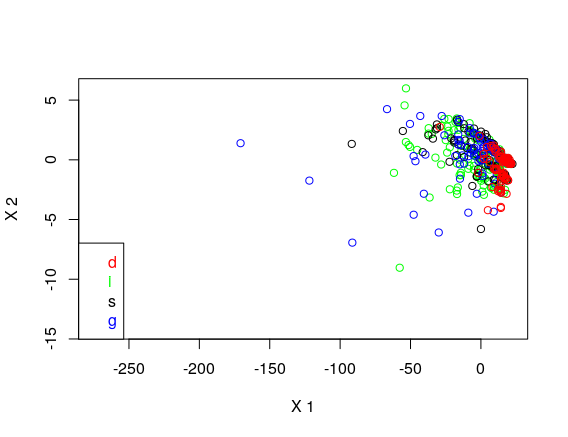
\includegraphics[scale=0.36]{PCA_1_2.png}
 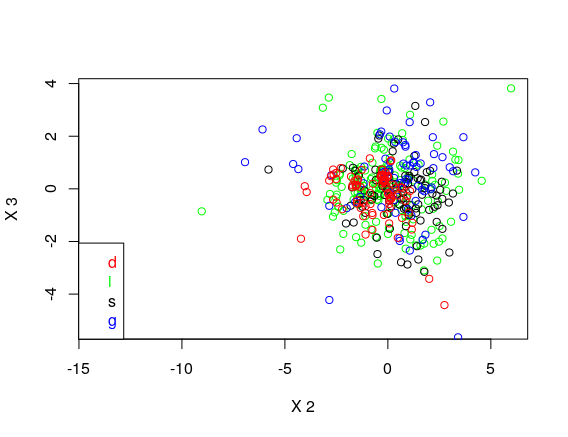
\includegraphics[scale=0.36]{PCA_2_3.png}
 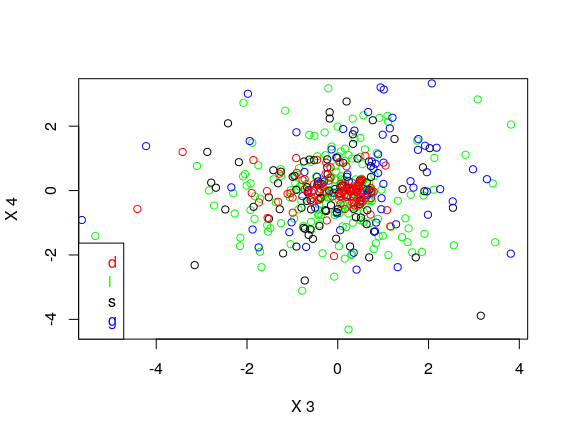
\includegraphics[scale=0.36]{PCA_3_4.png}
 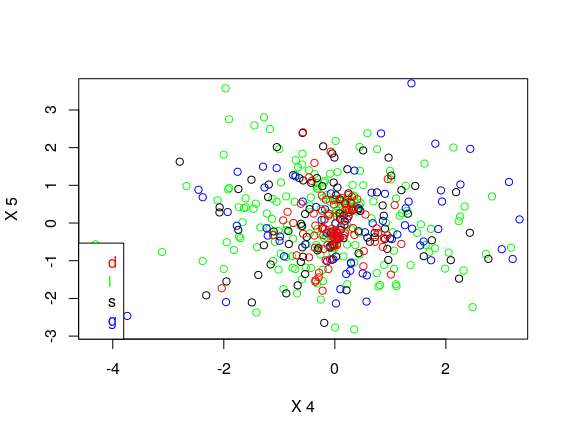
\includegraphics[scale=0.36]{PCA_4_5.png}
 
\end{frame}

\begin{frame}
 \frametitle{Erstellen von Prädiktoren}
 \framesubtitle{PCA - Principal Component Analysis}
 Fazit:
 \begin{itemize}
  \item Die Dominanten Reviews haben eine geringere Varianz
  \item keine erkennbaren Gruppen
  \item Mittelwerte der Gruppen sind ähnlich
 \end{itemize}
 
 Das Verfahren liefert keine besseren Ergebnisse und benötigt nicht wesentlich weniger Variablen. 

\end{frame}